\section{Design}

This section provides an overview of the design aspects of our tool during the first sprint. It includes diagrams that illustrate the system's structure and behavior.

\subsection{Class Diagram}

The class diagram (Figure \ref{fig:Sprint 1 Class Diagram}) visualizes the system's structure. It shows the classes, their attributes and operations, and the relationships among them.

\begin{figure}[ht]
	\centering
	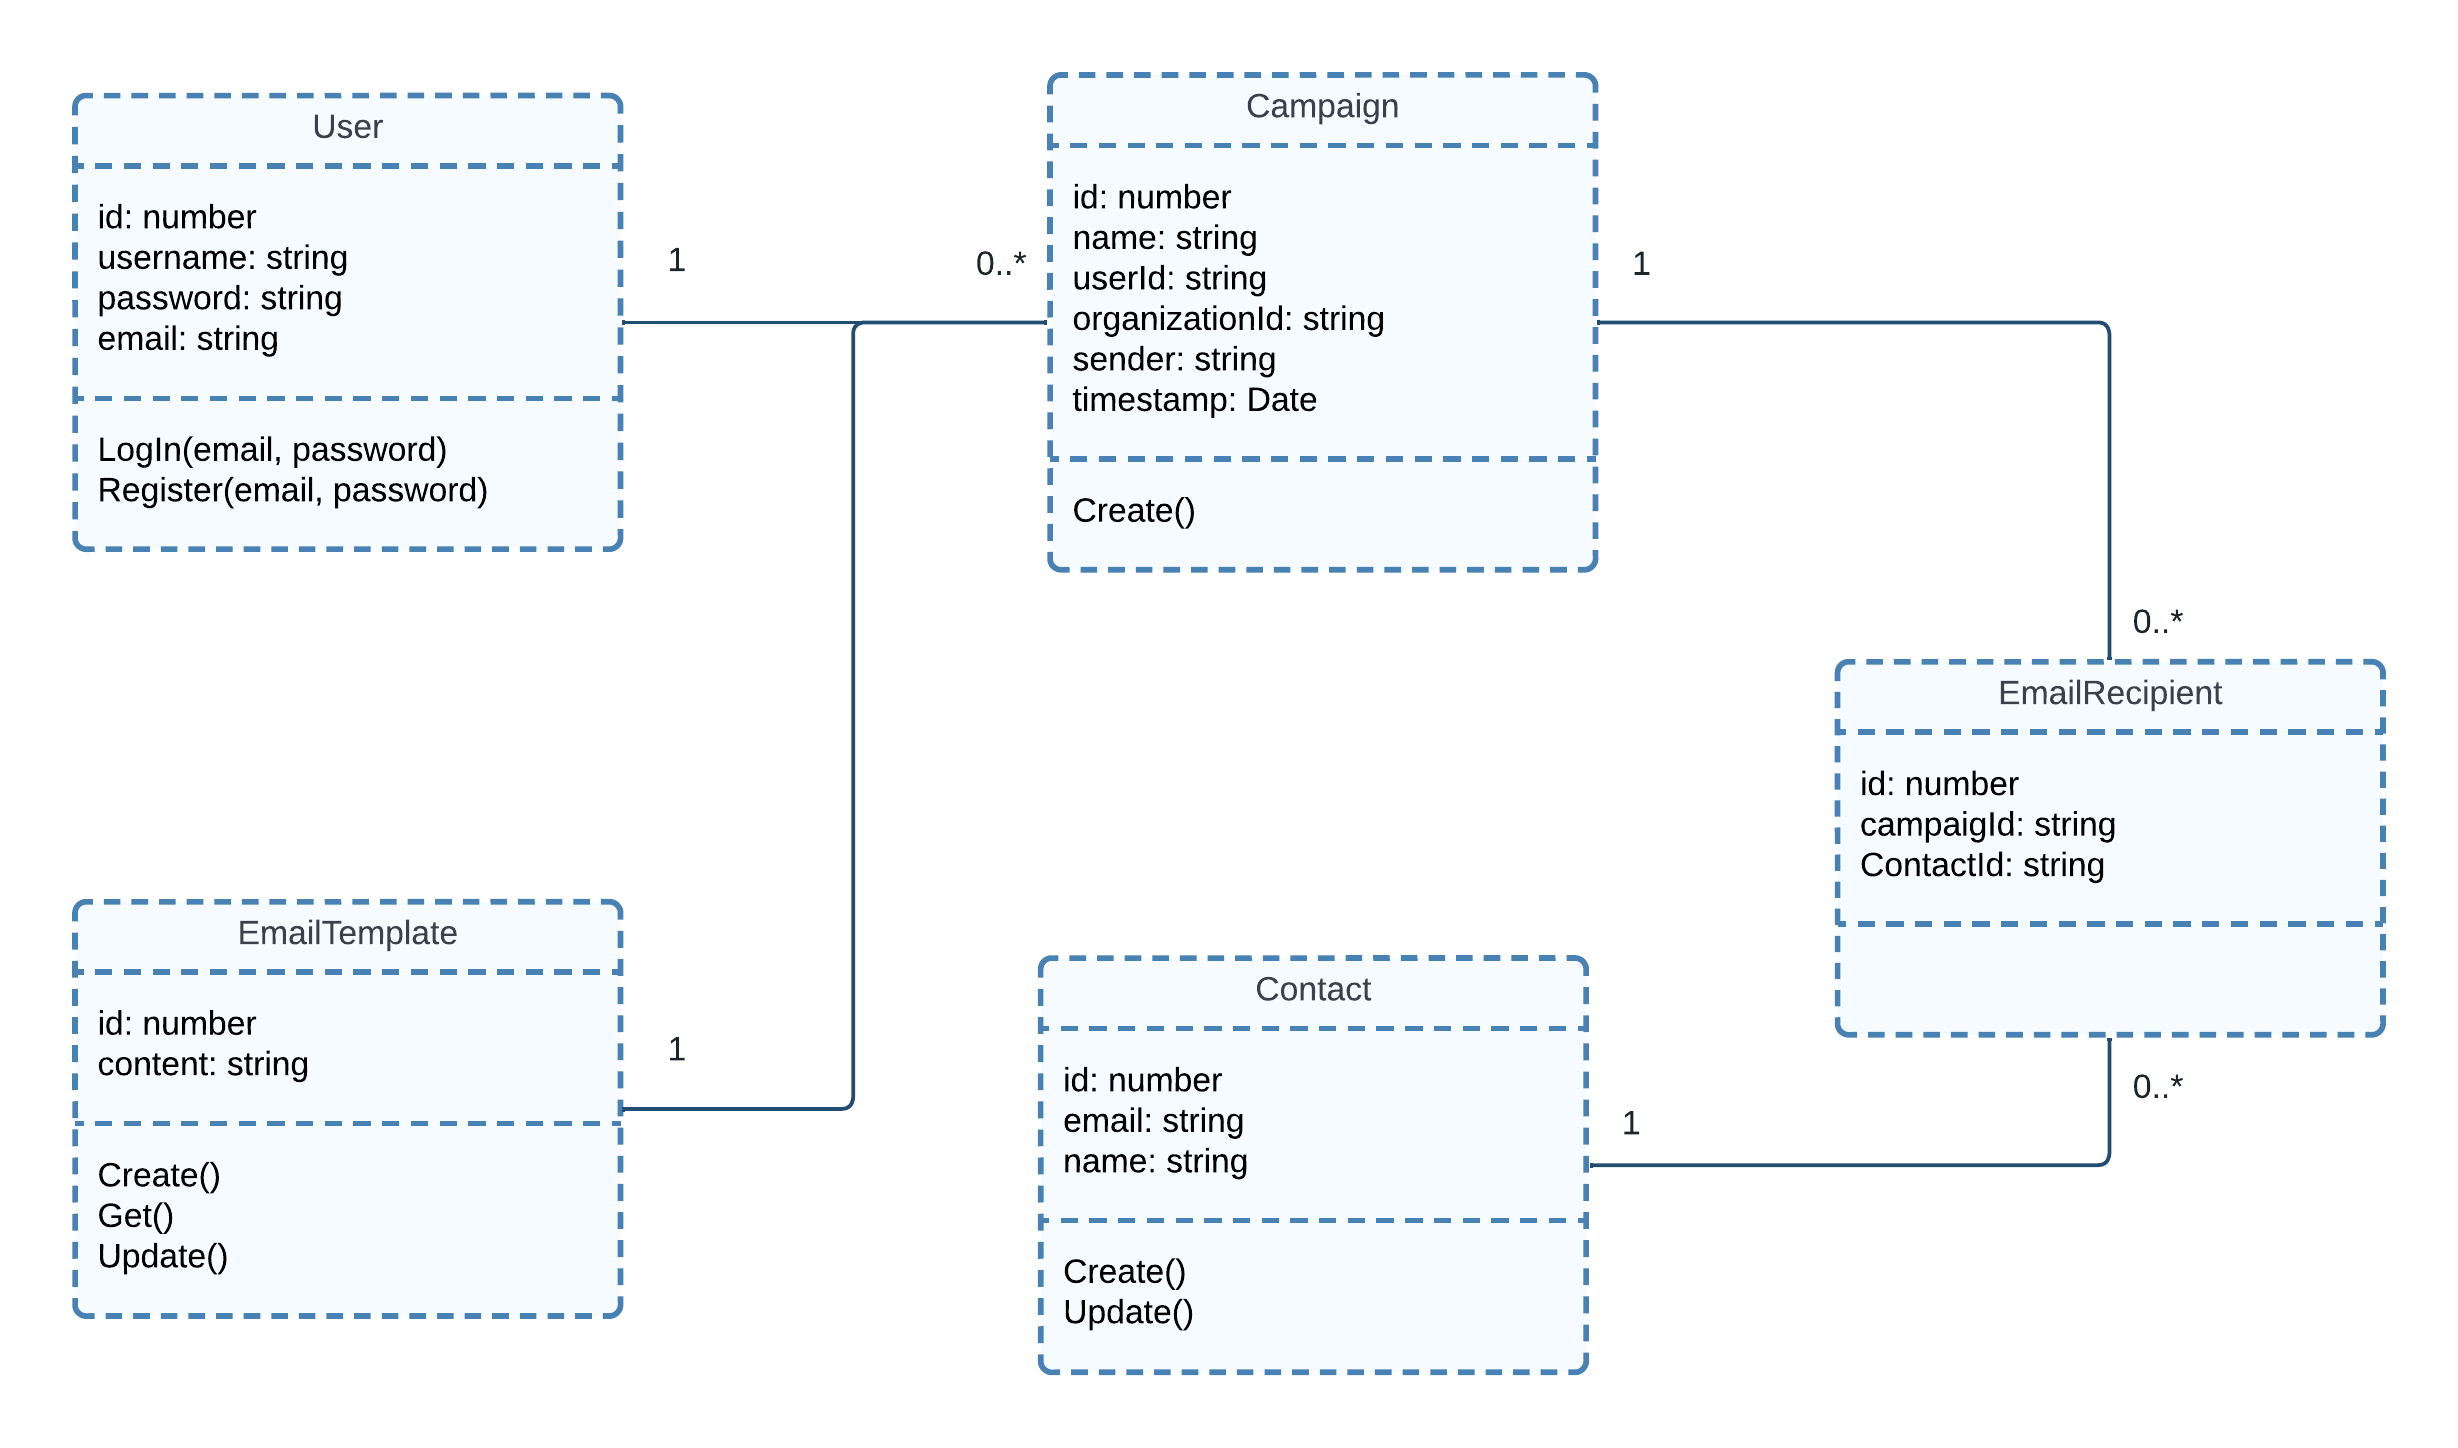
\includegraphics[width=\linewidth]{Images/Sprint1/class_diag_sprint_1.png}
	\caption{Sprint 1 Class Diagram}
	\label{fig:Sprint 1 Class Diagram}
\end{figure}


\clearpage

\subsection{Sequence Diagrams}

The sequence diagrams illustrate the flow of operations in the system, emphasizing the interaction between objects over time. Each diagram corresponds to a specific use case or functionality.

\subsubsection{Log In Sequence Diagram}

Figure \ref{fig:Sprint 1 Login Sequence Diagram} describes the scenario of the "Log In" use case.

\begin{figure}[ht]
	\centering
	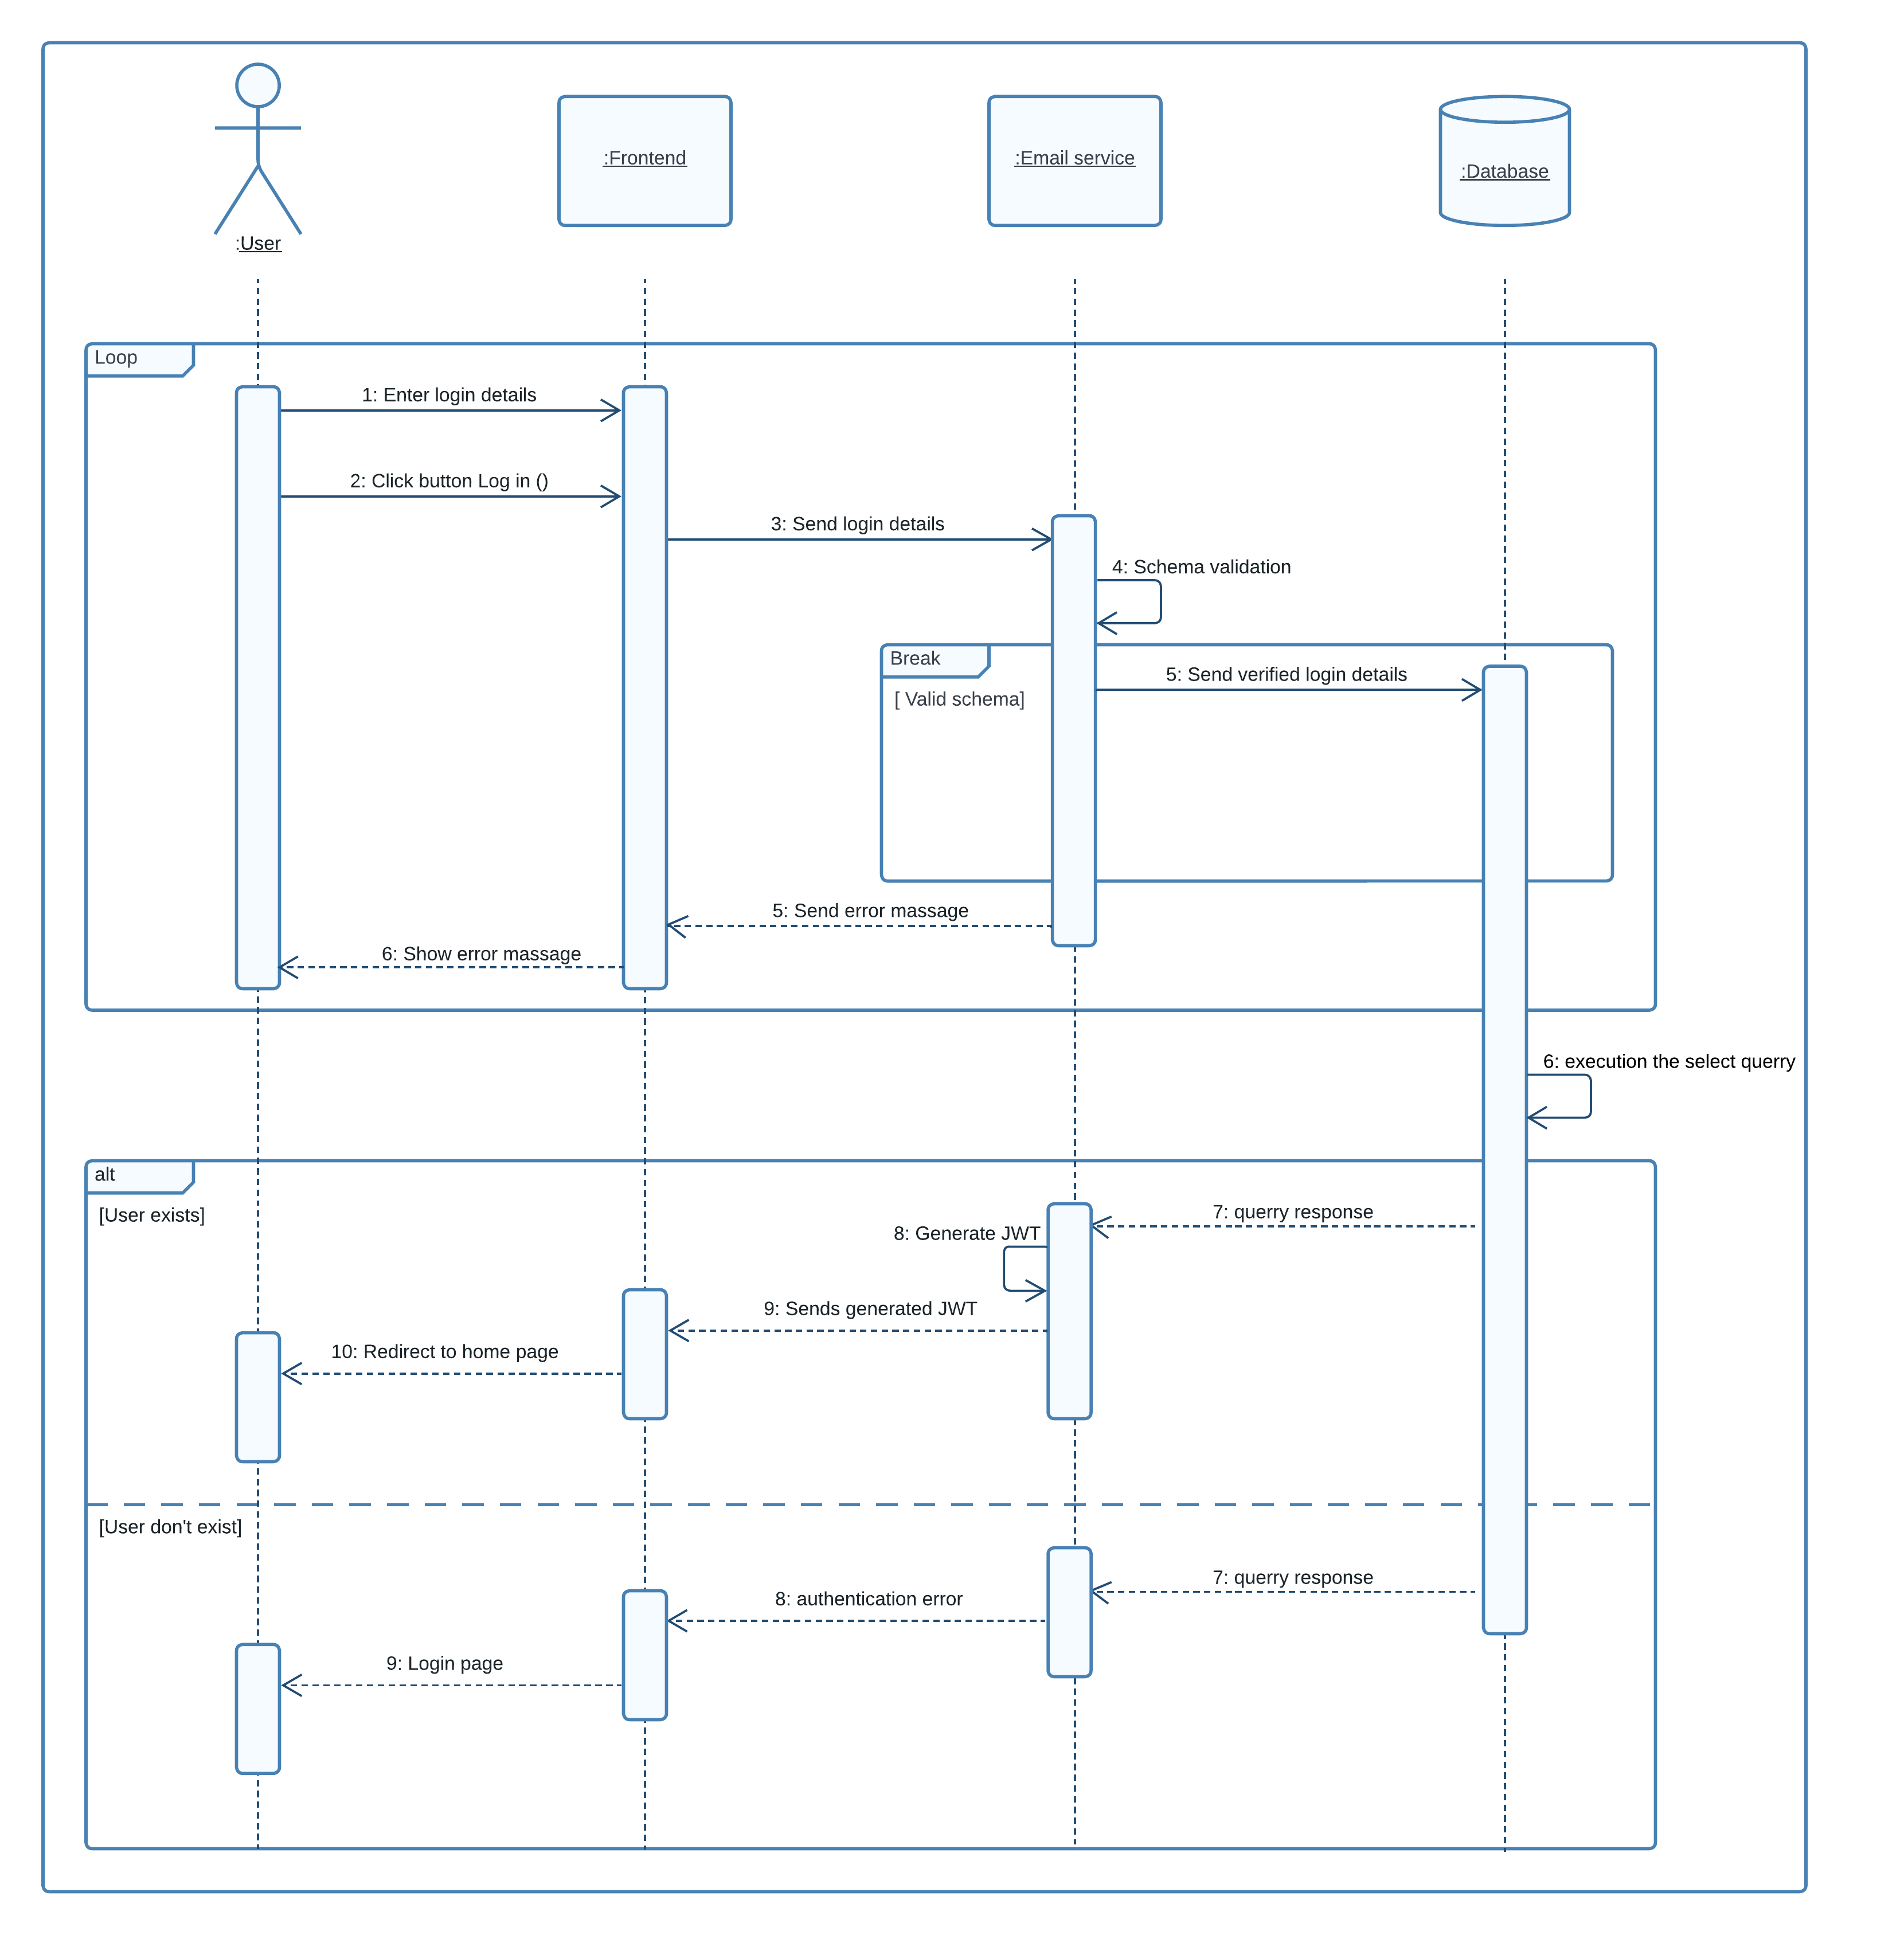
\includegraphics[width=\linewidth]{Images/Sprint1/sequence diagram sprint 1/auth v1.png}
	\caption{ Log In Sequence Diagram}
	\label{fig:Sprint 1 Login Sequence Diagram}
\end{figure}

\clearpage

\subsubsection{Register Sequence Diagram}

Figure \ref{fig:Sprint 1 Register Sequence Diagram} describes the scenario of the "Register" use case.

\begin{figure}[ht]
	\centering
	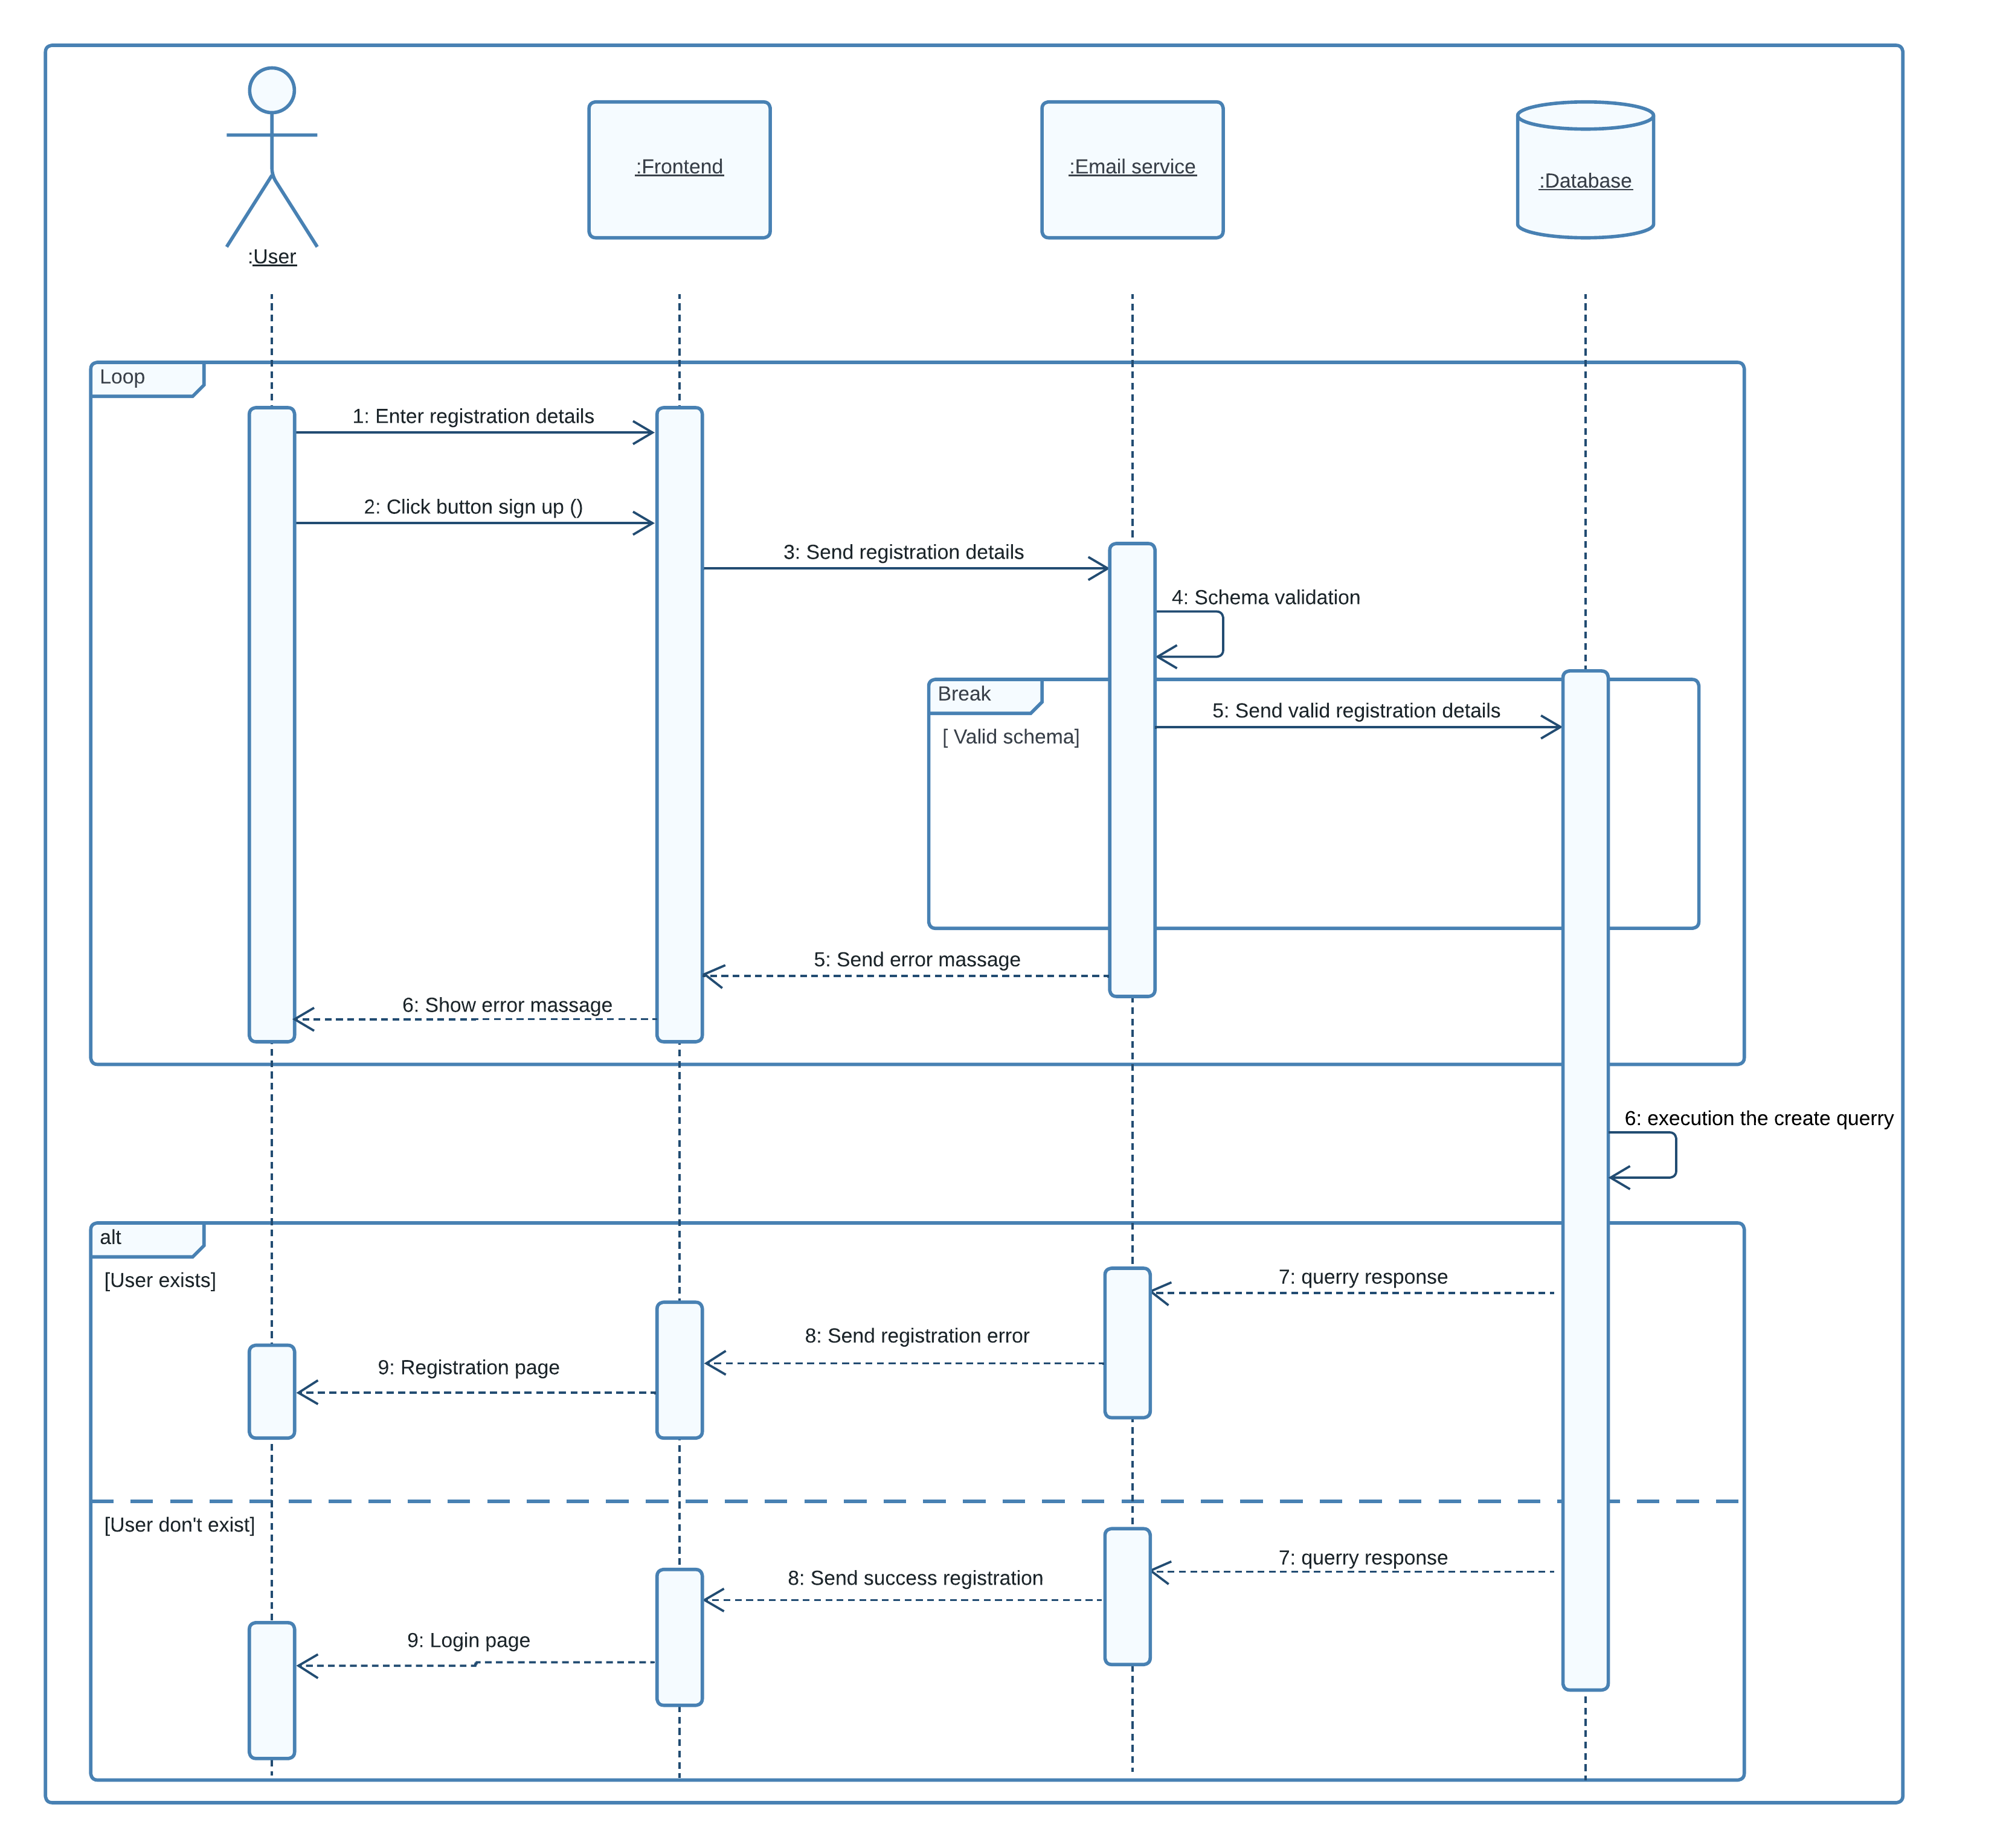
\includegraphics[width=\linewidth]{Images/Sprint1/sequence diagram sprint 1/register v3.png}
	\caption{ Register Sequence Diagram}
	\label{fig:Sprint 1 Register Sequence Diagram}
\end{figure}

\clearpage

\subsubsection{Create Email Template Sequence Diagram}

Figure \ref{fig:Sprint 1 Create Email Template Sequence Diagram} describes the scenario of the "Create Email Template" use case.

\begin{figure}[ht]
	\centering
	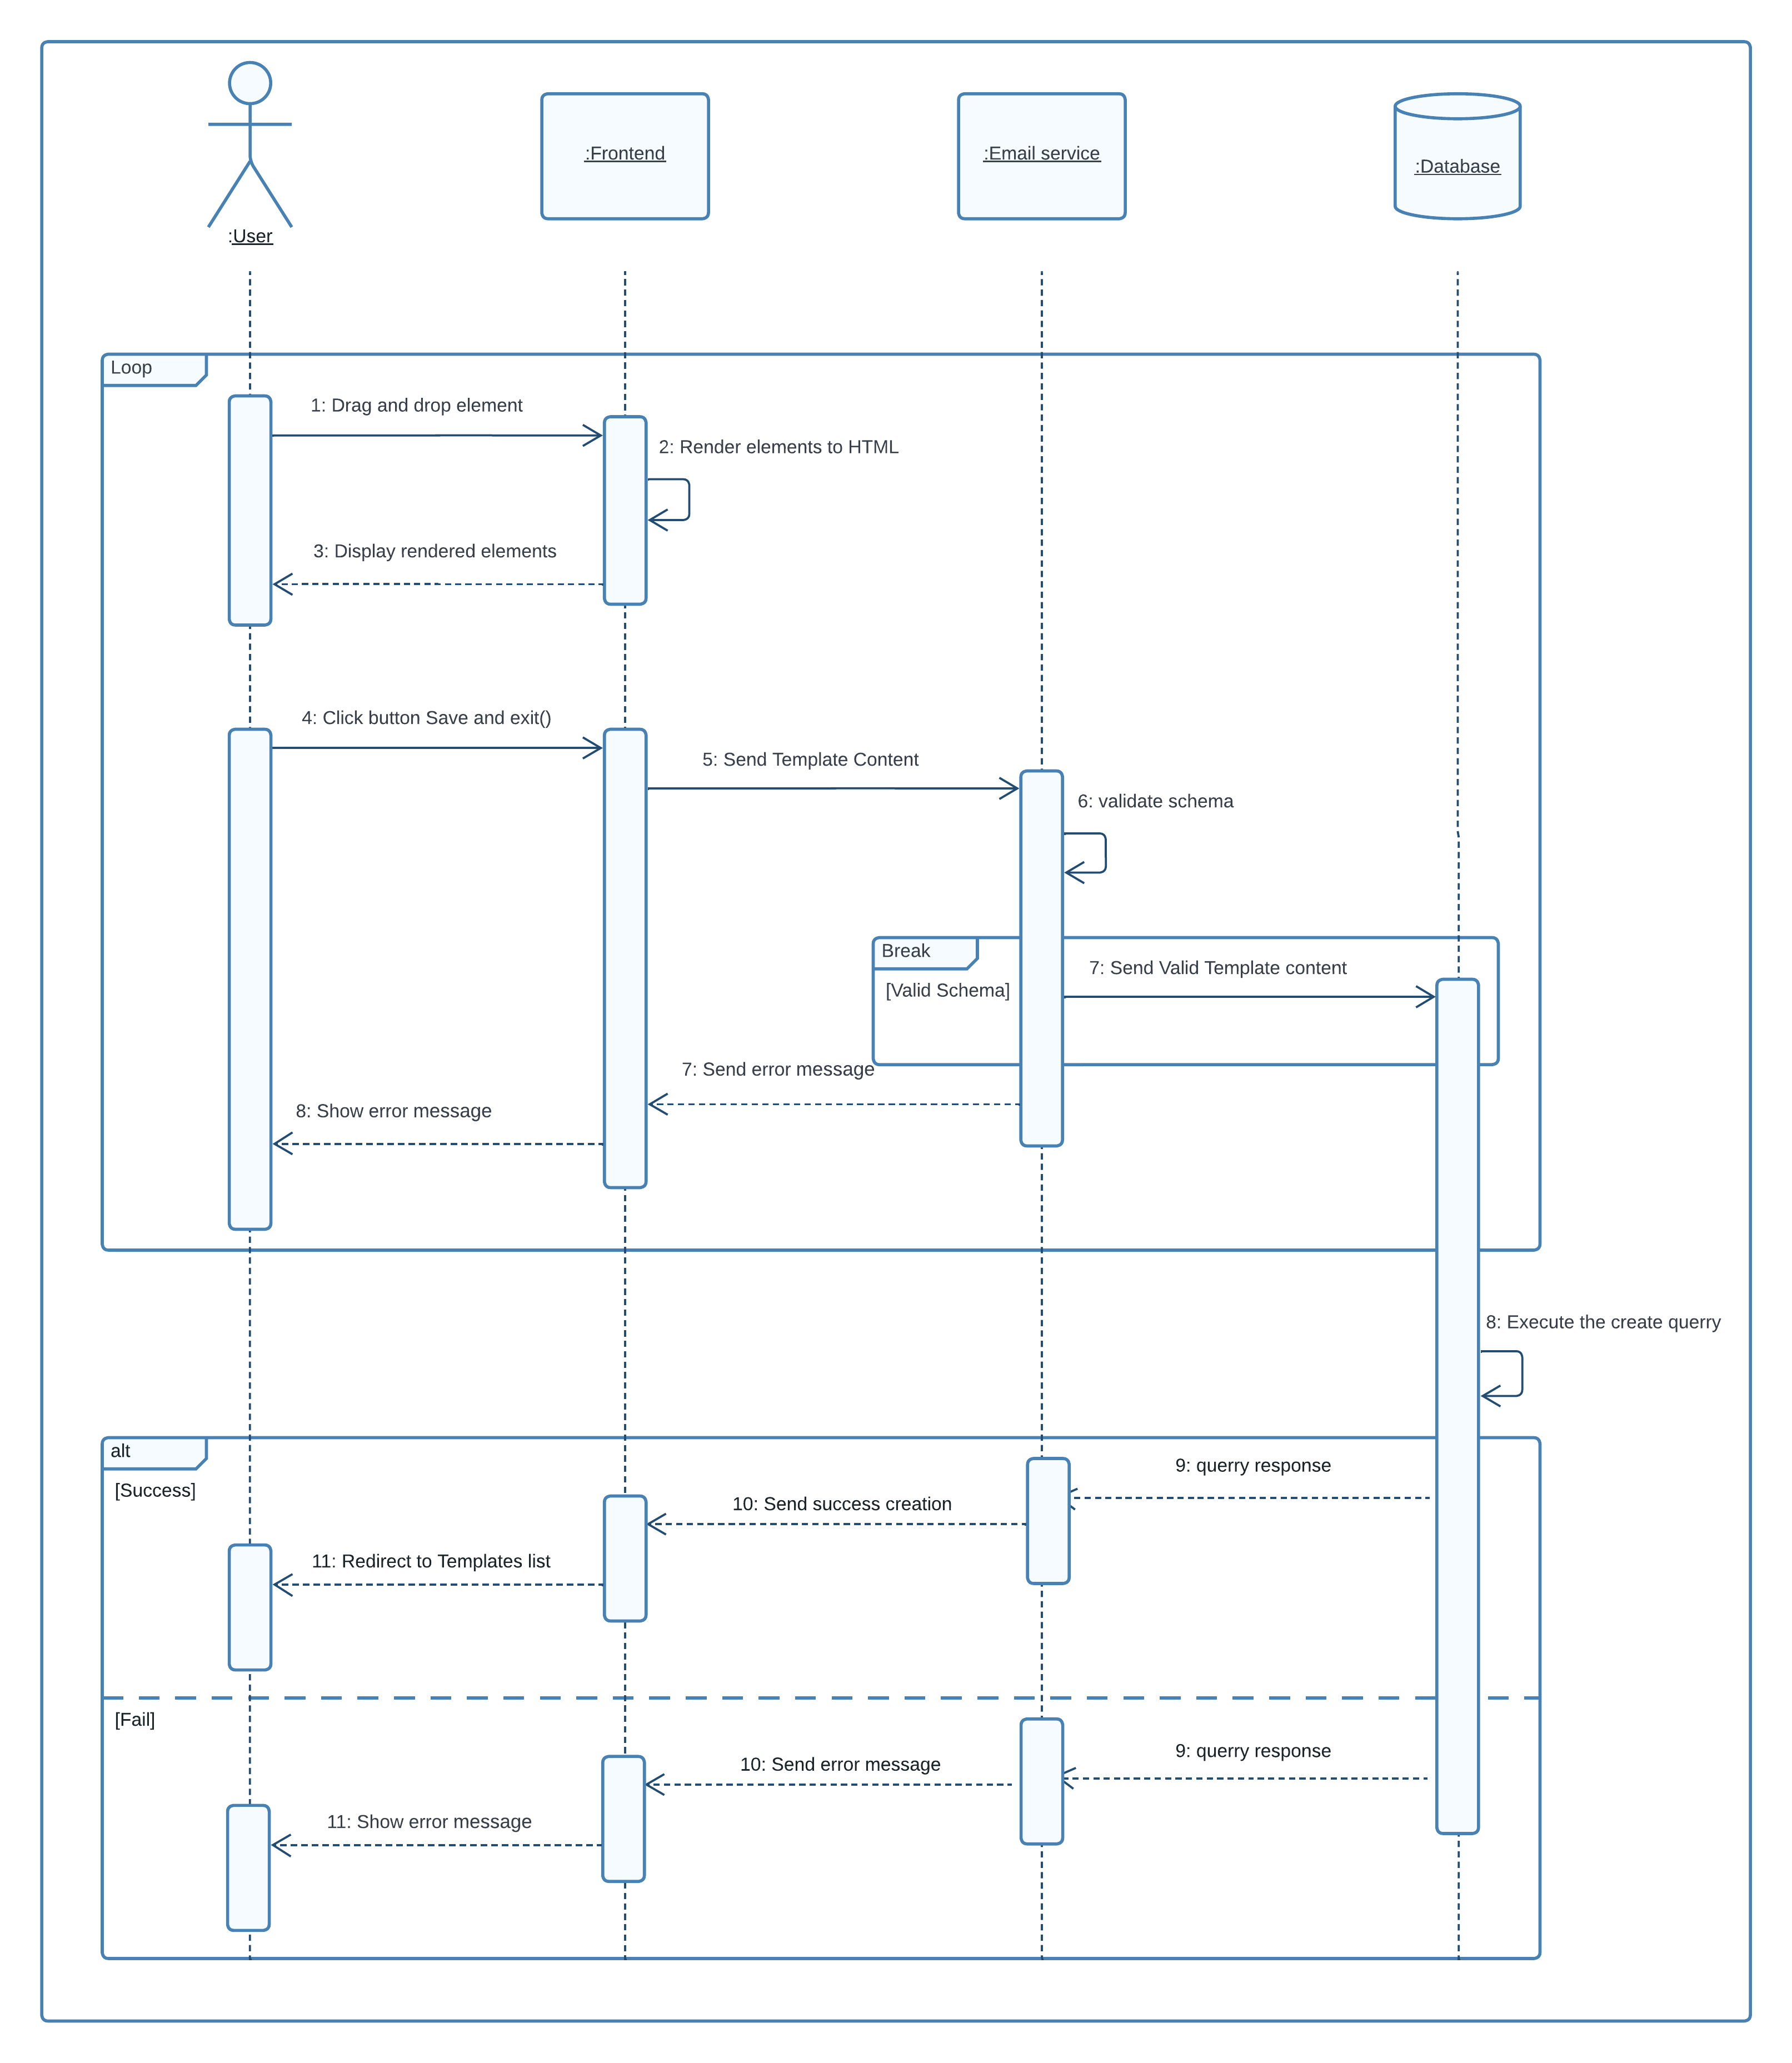
\includegraphics[width=\linewidth]{Images/Sprint1/sequence diagram sprint 1/email building v1.png}
	\caption{ Create Email Template Sequence Diagram}
	\label{fig:Sprint 1 Create Email Template Sequence Diagram}
\end{figure}

\clearpage

\subsubsection{Create And Publishing Campaigns Sequence Diagram}

Figure \ref{fig:Sprint 1 Create And Publishing Campaigns Sequence Diagram} describes the scenario of the "Create And Publishing Campaigns" use case.

\begin{figure}[ht]
	\centering
	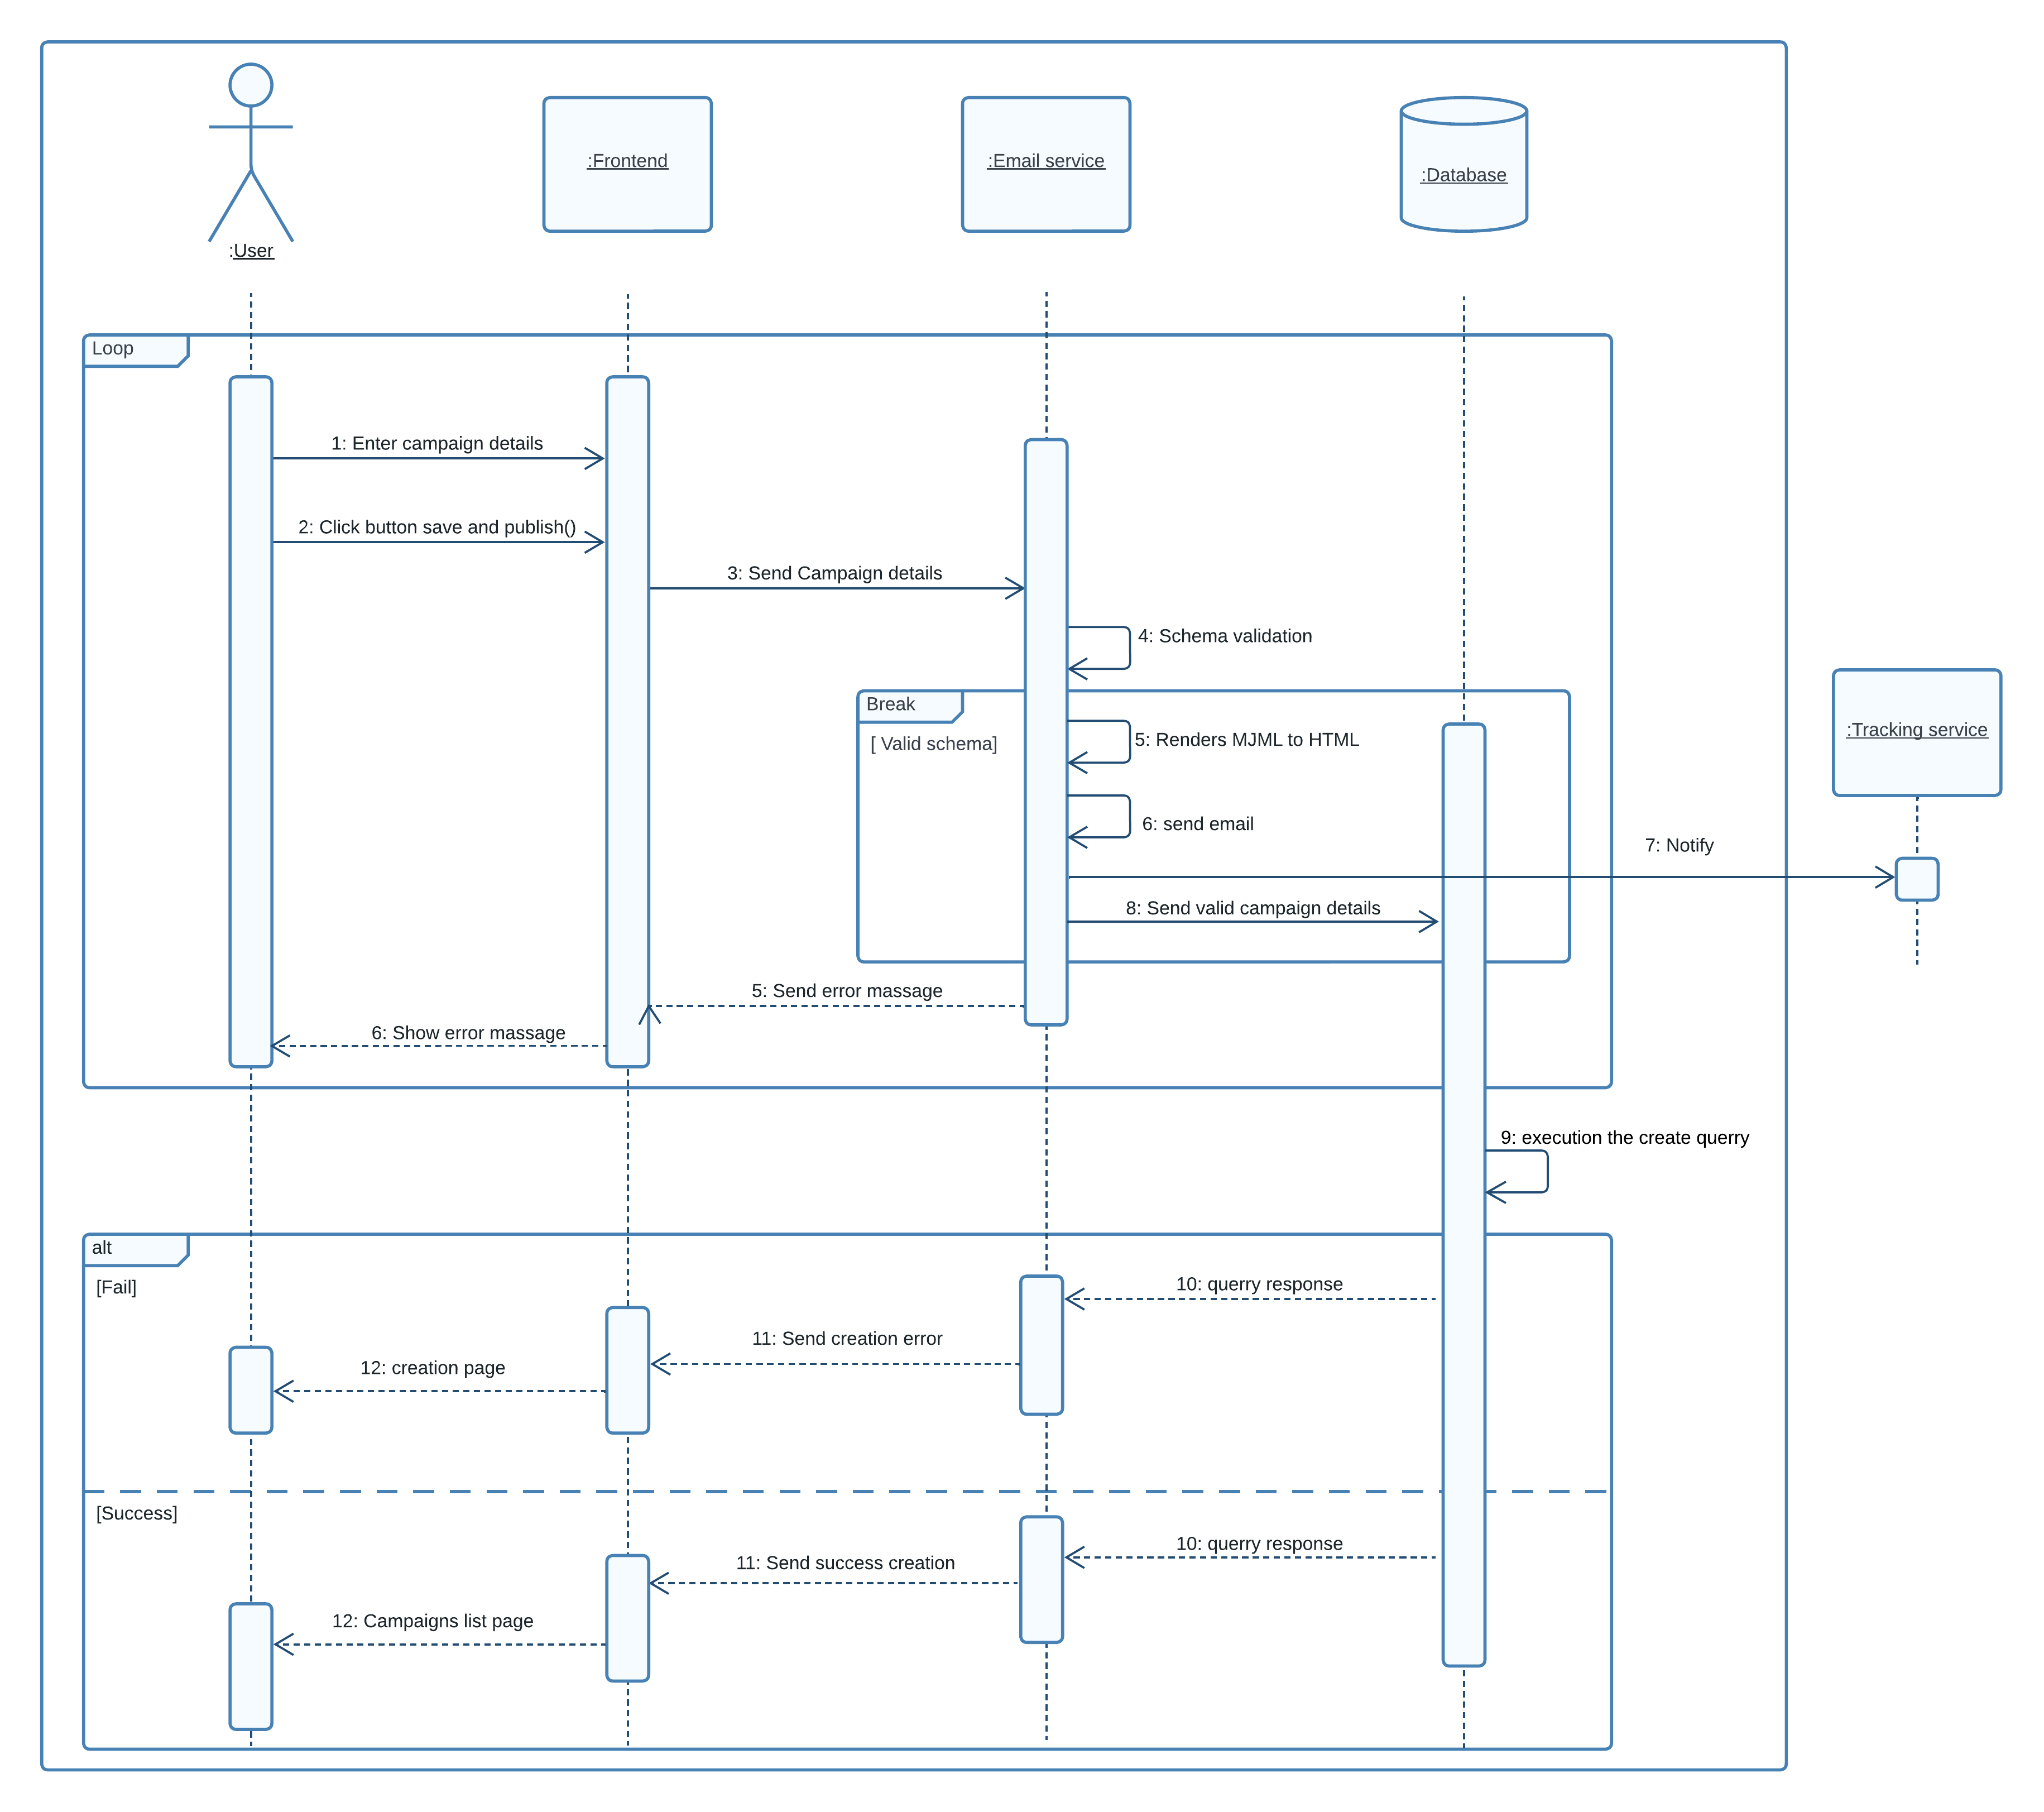
\includegraphics[width=\linewidth]{Images/Sprint1/sequence diagram sprint 1/campaign_creation.png}
	\caption{ Create And Publishing Campaigns Sequence Diagram}
	\label{fig:Sprint 1 Create And Publishing Campaigns Sequence Diagram}
\end{figure}

\clearpage

\subsubsection{Create Audience Sequence Diagram}

Figure \ref{fig:Sprint 1 Create Audience Sequence Diagram} describes the scenario of the "Create Audience" use case.

\begin{figure}[ht]
	\centering
	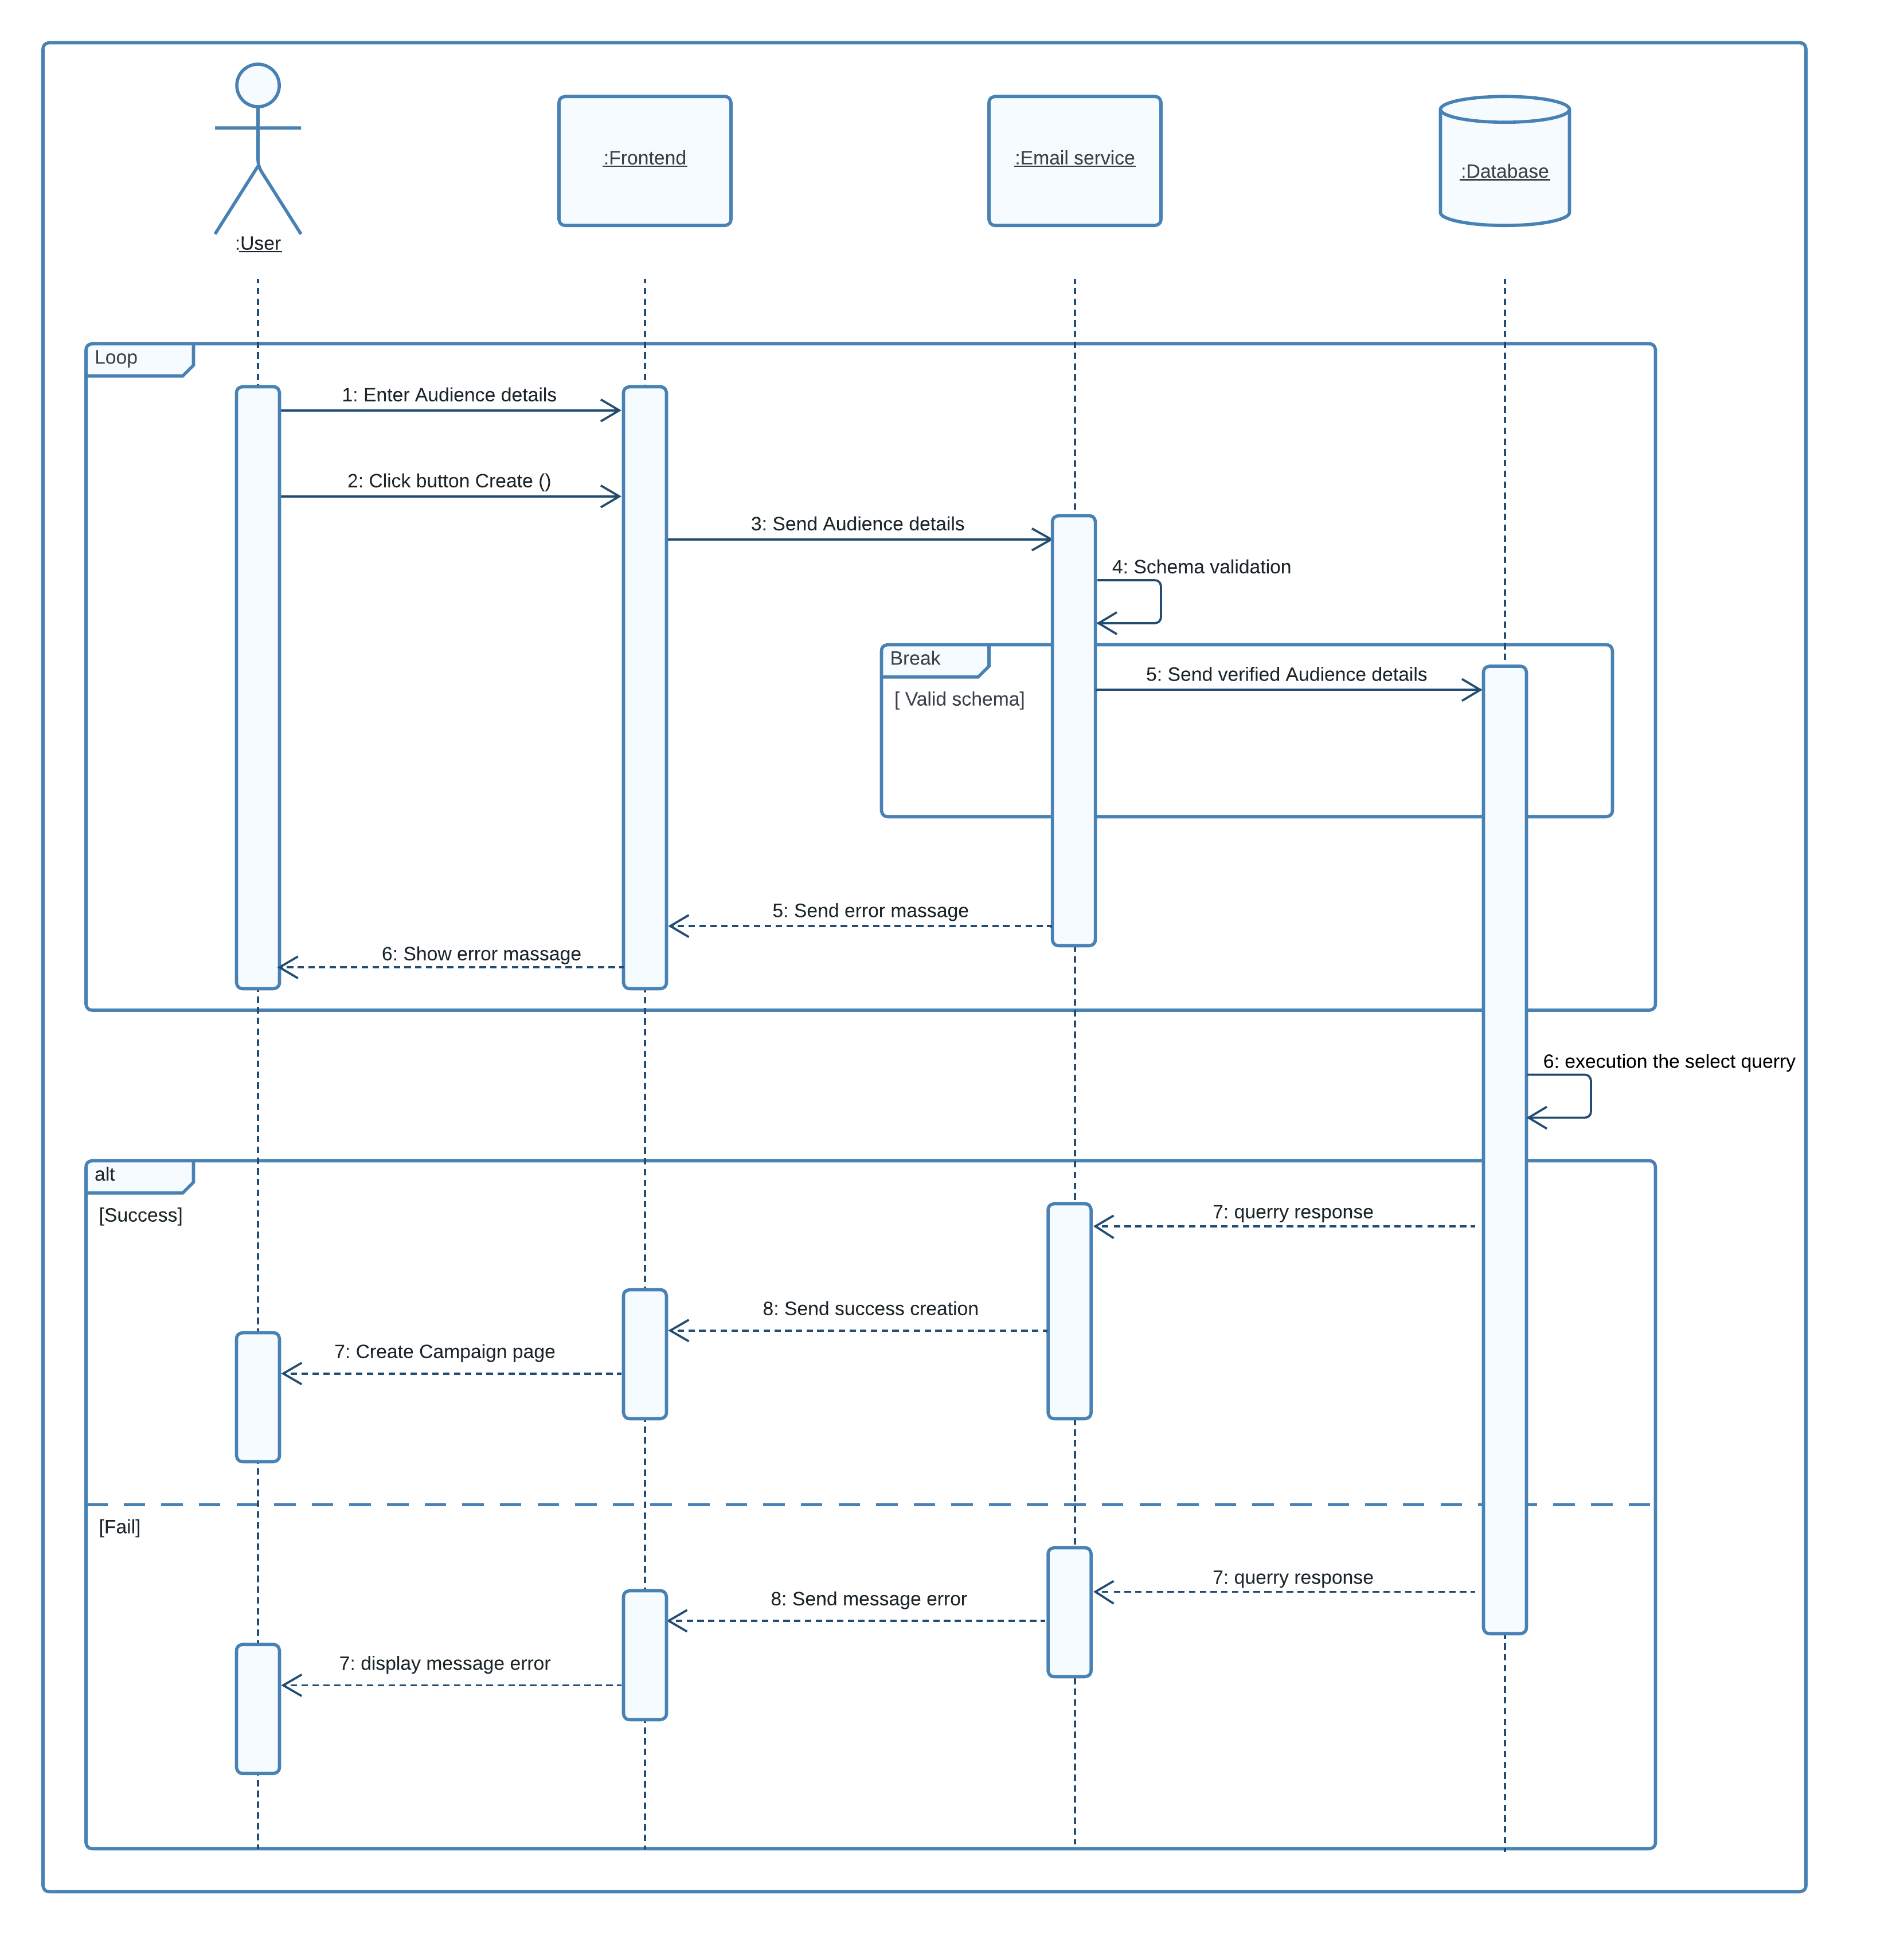
\includegraphics[width=\linewidth]{Images/Sprint1/sequence diagram sprint 1/create audience.png}
	\caption{ Create Audience Sequence Diagram }
	\label{fig:Sprint 1 Create Audience Sequence Diagram}
\end{figure}

\clearpage

